% Created by tikzDevice version 0.12.4 on 2023-08-26 16:37:00
% !TEX encoding = UTF-8 Unicode
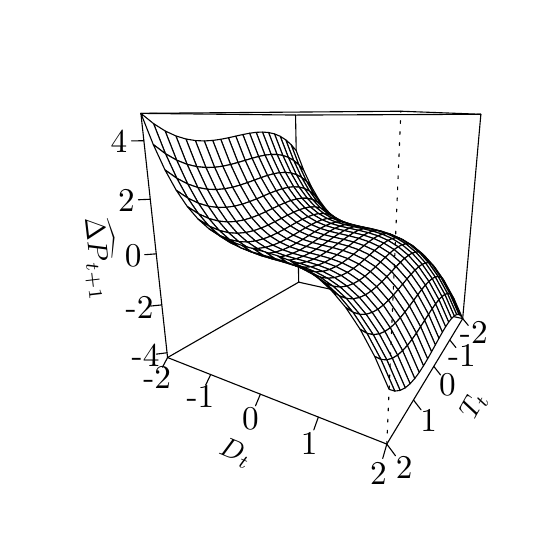
\begin{tikzpicture}[x=1pt,y=1pt]
\definecolor{fillColor}{RGB}{255,255,255}
\path[use as bounding box,fill=fillColor,fill opacity=0.00] (0,0) rectangle (180.67,180.67);
\begin{scope}
\path[clip] ( 36.00,  0.00) rectangle (168.67,180.67);
\definecolor{drawColor}{RGB}{0,0,0}

\path[draw=drawColor,line width= 0.4pt,line join=round,line cap=round] ( 97.94, 88.71) -- ( 96.79,149.09);

\path[draw=drawColor,line width= 0.4pt,line join=round,line cap=round] ( 96.79,149.09) -- ( 40.91,149.70);

\path[draw=drawColor,line width= 0.4pt,line join=round,line cap=round] ( 40.91,149.70) -- ( 50.55, 61.47);

\path[draw=drawColor,line width= 0.4pt,line join=round,line cap=round] ( 50.55, 61.47) -- ( 97.94, 88.71);

\path[draw=drawColor,line width= 0.4pt,line join=round,line cap=round] ( 97.94, 88.71) -- (157.19, 75.54);

\path[draw=drawColor,line width= 0.4pt,line join=round,line cap=round] (157.19, 75.54) -- (163.76,149.37);

\path[draw=drawColor,line width= 0.4pt,line join=round,line cap=round] (163.76,149.37) -- ( 96.79,149.09);

\path[draw=drawColor,line width= 0.4pt,line join=round,line cap=round] ( 50.55, 61.47) -- (129.77, 30.20);

\path[draw=drawColor,line width= 0.4pt,line join=round,line cap=round] (129.77, 30.20) -- (157.19, 75.54);

\path[draw=drawColor,line width= 0.4pt,line join=round,line cap=round] (163.76,149.37) -- (134.86,150.48);

\path[draw=drawColor,line width= 0.4pt,line join=round,line cap=round] (134.86,150.48) -- ( 40.91,149.70);
\end{scope}
\begin{scope}
\path[clip] (  0.00,  0.00) rectangle (180.67,180.67);
\definecolor{drawColor}{RGB}{0,0,0}

\node[text=drawColor,rotate= 60.83,anchor=base,inner sep=0pt, outer sep=0pt, scale=  1.00] at (153.16, 48.59) {};

\node[text=drawColor,rotate= 60.83,anchor=base,inner sep=0pt, outer sep=0pt, scale=  1.00] at (163.63, 42.74) { $T_{t}$};

\path[draw=drawColor,line width= 0.4pt,line join=round,line cap=round] (157.19, 75.54) -- (159.19, 73.10);

\node[text=drawColor,anchor=base,inner sep=0pt, outer sep=0pt, scale=  1.20] at (161.21, 66.51) {-2};

\path[draw=drawColor,line width= 0.4pt,line join=round,line cap=round] (152.52, 67.83) -- (154.73, 65.10);

\node[text=drawColor,anchor=base,inner sep=0pt, outer sep=0pt, scale=  1.20] at (156.95, 58.22) {-1};

\path[draw=drawColor,line width= 0.4pt,line join=round,line cap=round] (146.75, 58.28) -- (149.19, 55.18);

\node[text=drawColor,anchor=base,inner sep=0pt, outer sep=0pt, scale=  1.20] at (151.66, 47.93) {0};

\path[draw=drawColor,line width= 0.4pt,line join=round,line cap=round] (139.41, 46.14) -- (142.15, 42.57);

\node[text=drawColor,anchor=base,inner sep=0pt, outer sep=0pt, scale=  1.20] at (144.92, 34.84) {1};

\path[draw=drawColor,line width= 0.4pt,line join=round,line cap=round] (129.77, 30.20) -- (132.90, 25.99);

\node[text=drawColor,anchor=base,inner sep=0pt, outer sep=0pt, scale=  1.20] at (136.06, 17.60) {2};

\node[text=drawColor,rotate=-22.50,anchor=base,inner sep=0pt, outer sep=0pt, scale=  1.00] at ( 78.74, 35.52) {};

\node[text=drawColor,rotate=-22.50,anchor=base,inner sep=0pt, outer sep=0pt, scale=  1.00] at ( 74.15, 24.43) { $D_{t}$};

\path[draw=drawColor,line width= 0.4pt,line join=round,line cap=round] ( 50.55, 61.47) -- ( 48.70, 57.97);

\node[text=drawColor,anchor=base,inner sep=0pt, outer sep=0pt, scale=  1.20] at ( 46.82, 50.27) {-2};

\path[draw=drawColor,line width= 0.4pt,line join=round,line cap=round] ( 66.13, 55.32) -- ( 64.31, 51.50);

\node[text=drawColor,anchor=base,inner sep=0pt, outer sep=0pt, scale=  1.20] at ( 62.45, 43.48) {-1};

\path[draw=drawColor,line width= 0.4pt,line join=round,line cap=round] ( 84.09, 48.22) -- ( 82.33, 44.04);

\node[text=drawColor,anchor=base,inner sep=0pt, outer sep=0pt, scale=  1.20] at ( 80.53, 35.63) {0};

\path[draw=drawColor,line width= 0.4pt,line join=round,line cap=round] (105.04, 39.96) -- (103.38, 35.32);

\node[text=drawColor,anchor=base,inner sep=0pt, outer sep=0pt, scale=  1.20] at (101.69, 26.44) {1};

\path[draw=drawColor,line width= 0.4pt,line join=round,line cap=round] (129.77, 30.20) -- (128.29, 25.01);

\node[text=drawColor,anchor=base,inner sep=0pt, outer sep=0pt, scale=  1.20] at (126.77, 15.55) {2};

\node[text=drawColor,rotate=-83.36,anchor=base,inner sep=0pt, outer sep=0pt, scale=  1.00] at ( 34.27, 98.14) {};

\node[text=drawColor,rotate=-83.36,anchor=base,inner sep=0pt, outer sep=0pt, scale=  1.00] at ( 22.35, 96.75) { $\widehat{\Delta P}_{t+1}$};

\path[draw=drawColor,line width= 0.4pt,line join=round,line cap=round] ( 50.36, 63.20) -- ( 46.50, 62.70);

\node[text=drawColor,anchor=base,inner sep=0pt, outer sep=0pt, scale=  1.20] at ( 42.60, 58.07) {-4};

\path[draw=drawColor,line width= 0.4pt,line join=round,line cap=round] ( 48.47, 80.49) -- ( 44.47, 80.08);

\node[text=drawColor,anchor=base,inner sep=0pt, outer sep=0pt, scale=  1.20] at ( 40.43, 75.54) {-2};

\path[draw=drawColor,line width= 0.4pt,line join=round,line cap=round] ( 46.45, 98.94) -- ( 42.31, 98.63);

\node[text=drawColor,anchor=base,inner sep=0pt, outer sep=0pt, scale=  1.20] at ( 38.12, 94.19) {0};

\path[draw=drawColor,line width= 0.4pt,line join=round,line cap=round] ( 44.30,118.67) -- ( 40.00,118.48);

\node[text=drawColor,anchor=base,inner sep=0pt, outer sep=0pt, scale=  1.20] at ( 35.64,114.15) {2};

\path[draw=drawColor,line width= 0.4pt,line join=round,line cap=round] ( 41.99,139.81) -- ( 37.52,139.76);

\node[text=drawColor,anchor=base,inner sep=0pt, outer sep=0pt, scale=  1.20] at ( 32.99,135.57) {4};
\end{scope}
\begin{scope}
\path[clip] ( 36.00,  0.00) rectangle (168.67,180.67);
\definecolor{drawColor}{RGB}{0,0,0}
\definecolor{fillColor}{RGB}{255,255,255}

\path[draw=drawColor,line width= 0.4pt,line join=round,line cap=round,fill=fillColor] ( 97.03,136.24) --
	( 95.17,138.43) --
	( 97.98,131.11) --
	( 99.78,129.08) --
	cycle;

\path[draw=drawColor,line width= 0.4pt,line join=round,line cap=round,fill=fillColor] ( 99.78,129.08) --
	( 97.98,131.11) --
	(100.77,125.14) --
	(102.51,123.23) --
	cycle;

\path[draw=drawColor,line width= 0.4pt,line join=round,line cap=round,fill=fillColor] ( 95.17,138.43) --
	( 93.24,140.15) --
	( 96.12,132.68) --
	( 97.98,131.11) --
	cycle;

\path[draw=drawColor,line width= 0.4pt,line join=round,line cap=round,fill=fillColor] (102.51,123.23) --
	(100.77,125.14) --
	(103.55,120.33) --
	(105.23,118.52) --
	cycle;

\path[draw=drawColor,line width= 0.4pt,line join=round,line cap=round,fill=fillColor] ( 97.98,131.11) --
	( 96.12,132.68) --
	( 98.96,126.58) --
	(100.77,125.14) --
	cycle;

\path[draw=drawColor,line width= 0.4pt,line join=round,line cap=round,fill=fillColor] (105.23,118.52) --
	(103.55,120.33) --
	(106.33,116.53) --
	(107.97,114.79) --
	cycle;

\path[draw=drawColor,line width= 0.4pt,line join=round,line cap=round,fill=fillColor] ( 93.24,140.15) --
	( 91.25,141.42) --
	( 94.19,133.79) --
	( 96.12,132.68) --
	cycle;

\path[draw=drawColor,line width= 0.4pt,line join=round,line cap=round,fill=fillColor] (100.77,125.14) --
	( 98.96,126.58) --
	(101.79,121.67) --
	(103.55,120.33) --
	cycle;

\path[draw=drawColor,line width= 0.4pt,line join=round,line cap=round,fill=fillColor] (107.97,114.79) --
	(106.33,116.53) --
	(109.14,113.58) --
	(110.73,111.89) --
	cycle;

\path[draw=drawColor,line width= 0.4pt,line join=round,line cap=round,fill=fillColor] ( 96.12,132.68) --
	( 94.19,133.79) --
	( 97.09,127.57) --
	( 98.96,126.58) --
	cycle;

\path[draw=drawColor,line width= 0.4pt,line join=round,line cap=round,fill=fillColor] (103.55,120.33) --
	(101.79,121.67) --
	(104.63,117.79) --
	(106.33,116.53) --
	cycle;

\path[draw=drawColor,line width= 0.4pt,line join=round,line cap=round,fill=fillColor] (110.73,111.89) --
	(109.14,113.58) --
	(111.99,111.35) --
	(113.53,109.70) --
	cycle;

\path[draw=drawColor,line width= 0.4pt,line join=round,line cap=round,fill=fillColor] ( 91.25,141.42) --
	( 89.18,142.29) --
	( 92.19,134.50) --
	( 94.19,133.79) --
	cycle;

\path[draw=drawColor,line width= 0.4pt,line join=round,line cap=round,fill=fillColor] ( 98.96,126.58) --
	( 97.09,127.57) --
	( 99.97,122.57) --
	(101.79,121.67) --
	cycle;

\path[draw=drawColor,line width= 0.4pt,line join=round,line cap=round,fill=fillColor] (106.33,116.53) --
	(104.63,117.79) --
	(107.49,114.79) --
	(109.14,113.58) --
	cycle;

\path[draw=drawColor,line width= 0.4pt,line join=round,line cap=round,fill=fillColor] (113.53,109.70) --
	(111.99,111.35) --
	(114.89,109.70) --
	(116.37,108.07) --
	cycle;

\path[draw=drawColor,line width= 0.4pt,line join=round,line cap=round,fill=fillColor] ( 94.19,133.79) --
	( 92.19,134.50) --
	( 95.14,128.16) --
	( 97.09,127.57) --
	cycle;

\path[draw=drawColor,line width= 0.4pt,line join=round,line cap=round,fill=fillColor] (101.79,121.67) --
	( 99.97,122.57) --
	(102.86,118.61) --
	(104.63,117.79) --
	cycle;

\path[draw=drawColor,line width= 0.4pt,line join=round,line cap=round,fill=fillColor] (109.14,113.58) --
	(107.49,114.79) --
	(110.39,112.52) --
	(111.99,111.35) --
	cycle;

\path[draw=drawColor,line width= 0.4pt,line join=round,line cap=round,fill=fillColor] ( 89.18,142.29) --
	( 87.05,142.78) --
	( 90.11,134.84) --
	( 92.19,134.50) --
	cycle;

\path[draw=drawColor,line width= 0.4pt,line join=round,line cap=round,fill=fillColor] (116.37,108.07) --
	(114.89,109.70) --
	(117.84,108.50) --
	(119.27,106.88) --
	cycle;

\path[draw=drawColor,line width= 0.4pt,line join=round,line cap=round,fill=fillColor] ( 97.09,127.57) --
	( 95.14,128.16) --
	( 98.08,123.05) --
	( 99.97,122.57) --
	cycle;

\path[draw=drawColor,line width= 0.4pt,line join=round,line cap=round,fill=fillColor] (104.63,117.79) --
	(102.86,118.61) --
	(105.77,115.55) --
	(107.49,114.79) --
	cycle;

\path[draw=drawColor,line width= 0.4pt,line join=round,line cap=round,fill=fillColor] (111.99,111.35) --
	(110.39,112.52) --
	(113.33,110.85) --
	(114.89,109.70) --
	cycle;

\path[draw=drawColor,line width= 0.4pt,line join=round,line cap=round,fill=fillColor] ( 92.19,134.50) --
	( 90.11,134.84) --
	( 93.13,128.37) --
	( 95.14,128.16) --
	cycle;

\path[draw=drawColor,line width= 0.4pt,line join=round,line cap=round,fill=fillColor] (119.27,106.88) --
	(117.84,108.50) --
	(120.85,107.61) --
	(122.23,106.00) --
	cycle;

\path[draw=drawColor,line width= 0.4pt,line join=round,line cap=round,fill=fillColor] ( 99.97,122.57) --
	( 98.08,123.05) --
	(101.02,119.02) --
	(102.86,118.61) --
	cycle;

\path[draw=drawColor,line width= 0.4pt,line join=round,line cap=round,fill=fillColor] (107.49,114.79) --
	(105.77,115.55) --
	(108.71,113.24) --
	(110.39,112.52) --
	cycle;

\path[draw=drawColor,line width= 0.4pt,line join=round,line cap=round,fill=fillColor] ( 87.05,142.78) --
	( 84.84,142.95) --
	( 87.97,134.86) --
	( 90.11,134.84) --
	cycle;

\path[draw=drawColor,line width= 0.4pt,line join=round,line cap=round,fill=fillColor] (114.89,109.70) --
	(113.33,110.85) --
	(116.33,109.63) --
	(117.84,108.50) --
	cycle;

\path[draw=drawColor,line width= 0.4pt,line join=round,line cap=round,fill=fillColor] ( 95.14,128.16) --
	( 93.13,128.37) --
	( 96.12,123.17) --
	( 98.08,123.05) --
	cycle;

\path[draw=drawColor,line width= 0.4pt,line join=round,line cap=round,fill=fillColor] (122.23,106.00) --
	(120.85,107.61) --
	(123.92,106.90) --
	(125.25,105.29) --
	cycle;

\path[draw=drawColor,line width= 0.4pt,line join=round,line cap=round,fill=fillColor] (102.86,118.61) --
	(101.02,119.02) --
	(103.98,115.90) --
	(105.77,115.55) --
	cycle;

\path[draw=drawColor,line width= 0.4pt,line join=round,line cap=round,fill=fillColor] (110.39,112.52) --
	(108.71,113.24) --
	(111.70,111.54) --
	(113.33,110.85) --
	cycle;

\path[draw=drawColor,line width= 0.4pt,line join=round,line cap=round,fill=fillColor] ( 90.11,134.84) --
	( 87.97,134.86) --
	( 91.04,128.26) --
	( 93.13,128.37) --
	cycle;

\path[draw=drawColor,line width= 0.4pt,line join=round,line cap=round,fill=fillColor] (117.84,108.50) --
	(116.33,109.63) --
	(119.39,108.73) --
	(120.85,107.61) --
	cycle;

\path[draw=drawColor,line width= 0.4pt,line join=round,line cap=round,fill=fillColor] ( 98.08,123.05) --
	( 96.12,123.17) --
	( 99.11,119.05) --
	(101.02,119.02) --
	cycle;

\path[draw=drawColor,line width= 0.4pt,line join=round,line cap=round,fill=fillColor] (125.25,105.29) --
	(123.92,106.90) --
	(127.06,106.23) --
	(128.33,104.61) --
	cycle;

\path[draw=drawColor,line width= 0.4pt,line join=round,line cap=round,fill=fillColor] (105.77,115.55) --
	(103.98,115.90) --
	(106.97,113.54) --
	(108.71,113.24) --
	cycle;

\path[draw=drawColor,line width= 0.4pt,line join=round,line cap=round,fill=fillColor] ( 84.84,142.95) --
	( 82.56,142.85) --
	( 85.75,134.60) --
	( 87.97,134.86) --
	cycle;

\path[draw=drawColor,line width= 0.4pt,line join=round,line cap=round,fill=fillColor] (113.33,110.85) --
	(111.70,111.54) --
	(114.75,110.30) --
	(116.33,109.63) --
	cycle;

\path[draw=drawColor,line width= 0.4pt,line join=round,line cap=round,fill=fillColor] ( 93.13,128.37) --
	( 91.04,128.26) --
	( 94.09,122.95) --
	( 96.12,123.17) --
	cycle;

\path[draw=drawColor,line width= 0.4pt,line join=round,line cap=round,fill=fillColor] (120.85,107.61) --
	(119.39,108.73) --
	(122.52,108.02) --
	(123.92,106.90) --
	cycle;

\path[draw=drawColor,line width= 0.4pt,line join=round,line cap=round,fill=fillColor] (101.02,119.02) --
	( 99.11,119.05) --
	(102.12,115.87) --
	(103.98,115.90) --
	cycle;

\path[draw=drawColor,line width= 0.4pt,line join=round,line cap=round,fill=fillColor] (128.33,104.61) --
	(127.06,106.23) --
	(130.26,105.44) --
	(131.48,103.82) --
	cycle;

\path[draw=drawColor,line width= 0.4pt,line join=round,line cap=round,fill=fillColor] (108.71,113.24) --
	(106.97,113.54) --
	(110.01,111.81) --
	(111.70,111.54) --
	cycle;

\path[draw=drawColor,line width= 0.4pt,line join=round,line cap=round,fill=fillColor] ( 87.97,134.86) --
	( 85.75,134.60) --
	( 88.89,127.87) --
	( 91.04,128.26) --
	cycle;

\path[draw=drawColor,line width= 0.4pt,line join=round,line cap=round,fill=fillColor] (116.33,109.63) --
	(114.75,110.30) --
	(117.86,109.39) --
	(119.39,108.73) --
	cycle;

\path[draw=drawColor,line width= 0.4pt,line join=round,line cap=round,fill=fillColor] ( 96.12,123.17) --
	( 94.09,122.95) --
	( 97.13,118.75) --
	( 99.11,119.05) --
	cycle;

\path[draw=drawColor,line width= 0.4pt,line join=round,line cap=round,fill=fillColor] (123.92,106.90) --
	(122.52,108.02) --
	(125.72,107.34) --
	(127.06,106.23) --
	cycle;

\path[draw=drawColor,line width= 0.4pt,line join=round,line cap=round,fill=fillColor] (103.98,115.90) --
	(102.12,115.87) --
	(105.15,113.47) --
	(106.97,113.54) --
	cycle;

\path[draw=drawColor,line width= 0.4pt,line join=round,line cap=round,fill=fillColor] (131.48,103.82) --
	(130.26,105.44) --
	(133.52,104.39) --
	(134.67,102.78) --
	cycle;

\path[draw=drawColor,line width= 0.4pt,line join=round,line cap=round,fill=fillColor] ( 82.56,142.85) --
	( 80.19,142.53) --
	( 83.45,134.11) --
	( 85.75,134.60) --
	cycle;

\path[draw=drawColor,line width= 0.4pt,line join=round,line cap=round,fill=fillColor] (111.70,111.54) --
	(110.01,111.81) --
	(113.10,110.55) --
	(114.75,110.30) --
	cycle;

\path[draw=drawColor,line width= 0.4pt,line join=round,line cap=round,fill=fillColor] ( 91.04,128.26) --
	( 88.89,127.87) --
	( 91.98,122.45) --
	( 94.09,122.95) --
	cycle;

\path[draw=drawColor,line width= 0.4pt,line join=round,line cap=round,fill=fillColor] (119.39,108.73) --
	(117.86,109.39) --
	(121.04,108.67) --
	(122.52,108.02) --
	cycle;

\path[draw=drawColor,line width= 0.4pt,line join=round,line cap=round,fill=fillColor] ( 99.11,119.05) --
	( 97.13,118.75) --
	(100.18,115.51) --
	(102.12,115.87) --
	cycle;

\path[draw=drawColor,line width= 0.4pt,line join=round,line cap=round,fill=fillColor] (127.06,106.23) --
	(125.72,107.34) --
	(128.98,106.55) --
	(130.26,105.44) --
	cycle;

\path[draw=drawColor,line width= 0.4pt,line join=round,line cap=round,fill=fillColor] (106.97,113.54) --
	(105.15,113.47) --
	(108.24,111.69) --
	(110.01,111.81) --
	cycle;

\path[draw=drawColor,line width= 0.4pt,line join=round,line cap=round,fill=fillColor] (134.67,102.78) --
	(133.52,104.39) --
	(136.83,102.92) --
	(137.91,101.33) --
	cycle;

\path[draw=drawColor,line width= 0.4pt,line join=round,line cap=round,fill=fillColor] ( 85.75,134.60) --
	( 83.45,134.11) --
	( 86.65,127.25) --
	( 88.89,127.87) --
	cycle;

\path[draw=drawColor,line width= 0.4pt,line join=round,line cap=round,fill=fillColor] (114.75,110.30) --
	(113.10,110.55) --
	(116.26,109.62) --
	(117.86,109.39) --
	cycle;

\path[draw=drawColor,line width= 0.4pt,line join=round,line cap=round,fill=fillColor] ( 94.09,122.95) --
	( 91.98,122.45) --
	( 95.07,118.17) --
	( 97.13,118.75) --
	cycle;

\path[draw=drawColor,line width= 0.4pt,line join=round,line cap=round,fill=fillColor] (122.52,108.02) --
	(121.04,108.67) --
	(124.29,107.99) --
	(125.72,107.34) --
	cycle;

\path[draw=drawColor,line width= 0.4pt,line join=round,line cap=round,fill=fillColor] (102.12,115.87) --
	(100.18,115.51) --
	(103.27,113.05) --
	(105.15,113.47) --
	cycle;

\path[draw=drawColor,line width= 0.4pt,line join=round,line cap=round,fill=fillColor] (130.26,105.44) --
	(128.98,106.55) --
	(132.30,105.49) --
	(133.52,104.39) --
	cycle;

\path[draw=drawColor,line width= 0.4pt,line join=round,line cap=round,fill=fillColor] ( 80.19,142.53) --
	( 77.74,142.05) --
	( 81.07,133.47) --
	( 83.45,134.11) --
	cycle;

\path[draw=drawColor,line width= 0.4pt,line join=round,line cap=round,fill=fillColor] (110.01,111.81) --
	(108.24,111.69) --
	(111.38,110.41) --
	(113.10,110.55) --
	cycle;

\path[draw=drawColor,line width= 0.4pt,line join=round,line cap=round,fill=fillColor] (137.91,101.33) --
	(136.83,102.92) --
	(140.16,100.87) --
	(141.18, 99.32) --
	cycle;

\path[draw=drawColor,line width= 0.4pt,line join=round,line cap=round,fill=fillColor] ( 88.89,127.87) --
	( 86.65,127.25) --
	( 89.80,121.73) --
	( 91.98,122.45) --
	cycle;

\path[draw=drawColor,line width= 0.4pt,line join=round,line cap=round,fill=fillColor] (117.86,109.39) --
	(116.26,109.62) --
	(119.49,108.89) --
	(121.04,108.67) --
	cycle;

\path[draw=drawColor,line width= 0.4pt,line join=round,line cap=round,fill=fillColor] ( 97.13,118.75) --
	( 95.07,118.17) --
	( 98.17,114.86) --
	(100.18,115.51) --
	cycle;

\path[draw=drawColor,line width= 0.4pt,line join=round,line cap=round,fill=fillColor] (125.72,107.34) --
	(124.29,107.99) --
	(127.61,107.18) --
	(128.98,106.55) --
	cycle;

\path[draw=drawColor,line width= 0.4pt,line join=round,line cap=round,fill=fillColor] (105.15,113.47) --
	(103.27,113.05) --
	(106.40,111.24) --
	(108.24,111.69) --
	cycle;

\path[draw=drawColor,line width= 0.4pt,line join=round,line cap=round,fill=fillColor] (133.52,104.39) --
	(132.30,105.49) --
	(135.66,103.99) --
	(136.83,102.92) --
	cycle;

\path[draw=drawColor,line width= 0.4pt,line join=round,line cap=round,fill=fillColor] ( 83.45,134.11) --
	( 81.07,133.47) --
	( 84.32,126.47) --
	( 86.65,127.25) --
	cycle;

\path[draw=drawColor,line width= 0.4pt,line join=round,line cap=round,fill=fillColor] (113.10,110.55) --
	(111.38,110.41) --
	(114.59,109.46) --
	(116.26,109.62) --
	cycle;

\path[draw=drawColor,line width= 0.4pt,line join=round,line cap=round,fill=fillColor] (141.18, 99.32) --
	(140.16,100.87) --
	(143.51, 98.08) --
	(144.46, 96.58) --
	cycle;

\path[draw=drawColor,line width= 0.4pt,line join=round,line cap=round,fill=fillColor] ( 91.98,122.45) --
	( 89.80,121.73) --
	( 92.94,117.36) --
	( 95.07,118.17) --
	cycle;

\path[draw=drawColor,line width= 0.4pt,line join=round,line cap=round,fill=fillColor] (121.04,108.67) --
	(119.49,108.89) --
	(122.80,108.19) --
	(124.29,107.99) --
	cycle;

\path[draw=drawColor,line width= 0.4pt,line join=round,line cap=round,fill=fillColor] (100.18,115.51) --
	( 98.17,114.86) --
	(101.30,112.35) --
	(103.27,113.05) --
	cycle;

\path[draw=drawColor,line width= 0.4pt,line join=round,line cap=round,fill=fillColor] (128.98,106.55) --
	(127.61,107.18) --
	(130.99,106.10) --
	(132.30,105.49) --
	cycle;

\path[draw=drawColor,line width= 0.4pt,line join=round,line cap=round,fill=fillColor] ( 77.74,142.05) --
	( 75.19,141.48) --
	( 78.59,132.72) --
	( 81.07,133.47) --
	cycle;

\path[draw=drawColor,line width= 0.4pt,line join=round,line cap=round,fill=fillColor] (108.24,111.69) --
	(106.40,111.24) --
	(109.58,109.92) --
	(111.38,110.41) --
	cycle;

\path[draw=drawColor,line width= 0.4pt,line join=round,line cap=round,fill=fillColor] (136.83,102.92) --
	(135.66,103.99) --
	(139.07,101.91) --
	(140.16,100.87) --
	cycle;

\path[draw=drawColor,line width= 0.4pt,line join=round,line cap=round,fill=fillColor] ( 86.65,127.25) --
	( 84.32,126.47) --
	( 87.53,120.84) --
	( 89.80,121.73) --
	cycle;

\path[draw=drawColor,line width= 0.4pt,line join=round,line cap=round,fill=fillColor] (116.26,109.62) --
	(114.59,109.46) --
	(117.87,108.71) --
	(119.49,108.89) --
	cycle;

\path[draw=drawColor,line width= 0.4pt,line join=round,line cap=round,fill=fillColor] (144.46, 96.58) --
	(143.51, 98.08) --
	(146.85, 94.40) --
	(147.72, 92.98) --
	cycle;

\path[draw=drawColor,line width= 0.4pt,line join=round,line cap=round,fill=fillColor] ( 95.07,118.17) --
	( 92.94,117.36) --
	( 96.09,113.97) --
	( 98.17,114.86) --
	cycle;

\path[draw=drawColor,line width= 0.4pt,line join=round,line cap=round,fill=fillColor] (124.29,107.99) --
	(122.80,108.19) --
	(126.17,107.37) --
	(127.61,107.18) --
	cycle;

\path[draw=drawColor,line width= 0.4pt,line join=round,line cap=round,fill=fillColor] (103.27,113.05) --
	(101.30,112.35) --
	(104.48,110.49) --
	(106.40,111.24) --
	cycle;

\path[draw=drawColor,line width= 0.4pt,line join=round,line cap=round,fill=fillColor] (132.30,105.49) --
	(130.99,106.10) --
	(134.42,104.58) --
	(135.66,103.99) --
	cycle;

\path[draw=drawColor,line width= 0.4pt,line join=round,line cap=round,fill=fillColor] ( 81.07,133.47) --
	( 78.59,132.72) --
	( 81.91,125.58) --
	( 84.32,126.47) --
	cycle;

\path[draw=drawColor,line width= 0.4pt,line join=round,line cap=round,fill=fillColor] (111.38,110.41) --
	(109.58,109.92) --
	(112.84,108.95) --
	(114.59,109.46) --
	cycle;

\path[draw=drawColor,line width= 0.4pt,line join=round,line cap=round,fill=fillColor] (140.16,100.87) --
	(139.07,101.91) --
	(142.49, 99.06) --
	(143.51, 98.08) --
	cycle;

\path[draw=drawColor,line width= 0.4pt,line join=round,line cap=round,fill=fillColor] ( 89.80,121.73) --
	( 87.53,120.84) --
	( 90.73,116.37) --
	( 92.94,117.36) --
	cycle;

\path[draw=drawColor,line width= 0.4pt,line join=round,line cap=round,fill=fillColor] (119.49,108.89) --
	(117.87,108.71) --
	(121.22,107.99) --
	(122.80,108.19) --
	cycle;

\path[draw=drawColor,line width= 0.4pt,line join=round,line cap=round,fill=fillColor] (147.72, 92.98) --
	(146.85, 94.40) --
	(150.16, 89.67) --
	(150.95, 88.35) --
	cycle;

\path[draw=drawColor,line width= 0.4pt,line join=round,line cap=round,fill=fillColor] ( 98.17,114.86) --
	( 96.09,113.97) --
	( 99.26,111.40) --
	(101.30,112.35) --
	cycle;

\path[draw=drawColor,line width= 0.4pt,line join=round,line cap=round,fill=fillColor] (127.61,107.18) --
	(126.17,107.37) --
	(129.61,106.27) --
	(130.99,106.10) --
	cycle;

\path[draw=drawColor,line width= 0.4pt,line join=round,line cap=round,fill=fillColor] ( 75.19,141.48) --
	( 72.53,140.88) --
	( 76.01,131.95) --
	( 78.59,132.72) --
	cycle;

\path[draw=drawColor,line width= 0.4pt,line join=round,line cap=round,fill=fillColor] (106.40,111.24) --
	(104.48,110.49) --
	(107.71,109.14) --
	(109.58,109.92) --
	cycle;

\path[draw=drawColor,line width= 0.4pt,line join=round,line cap=round,fill=fillColor] (135.66,103.99) --
	(134.42,104.58) --
	(137.89,102.45) --
	(139.07,101.91) --
	cycle;

\path[draw=drawColor,line width= 0.4pt,line join=round,line cap=round,fill=fillColor] ( 84.32,126.47) --
	( 81.91,125.58) --
	( 85.18,119.83) --
	( 87.53,120.84) --
	cycle;

\path[draw=drawColor,line width= 0.4pt,line join=round,line cap=round,fill=fillColor] (114.59,109.46) --
	(112.84,108.95) --
	(116.17,108.18) --
	(117.87,108.71) --
	cycle;

\path[draw=drawColor,line width= 0.4pt,line join=round,line cap=round,fill=fillColor] (143.51, 98.08) --
	(142.49, 99.06) --
	(145.90, 95.29) --
	(146.85, 94.40) --
	cycle;

\path[draw=drawColor,line width= 0.4pt,line join=round,line cap=round,fill=fillColor] ( 92.94,117.36) --
	( 90.73,116.37) --
	( 93.92,112.91) --
	( 96.09,113.97) --
	cycle;

\path[draw=drawColor,line width= 0.4pt,line join=round,line cap=round,fill=fillColor] (122.80,108.19) --
	(121.22,107.99) --
	(124.65,107.15) --
	(126.17,107.37) --
	cycle;

\path[draw=drawColor,line width= 0.4pt,line join=round,line cap=round,fill=fillColor] (150.95, 88.35) --
	(150.16, 89.67) --
	(153.40, 83.76) --
	(154.12, 82.58) --
	cycle;

\path[draw=drawColor,line width= 0.4pt,line join=round,line cap=round,fill=fillColor] (101.30,112.35) --
	( 99.26,111.40) --
	(102.49,109.50) --
	(104.48,110.49) --
	cycle;

\path[draw=drawColor,line width= 0.4pt,line join=round,line cap=round,fill=fillColor] (130.99,106.10) --
	(129.61,106.27) --
	(133.10,104.72) --
	(134.42,104.58) --
	cycle;

\path[draw=drawColor,line width= 0.4pt,line join=round,line cap=round,fill=fillColor] ( 78.59,132.72) --
	( 76.01,131.95) --
	( 79.40,124.66) --
	( 81.91,125.58) --
	cycle;

\path[draw=drawColor,line width= 0.4pt,line join=round,line cap=round,fill=fillColor] (109.58,109.92) --
	(107.71,109.14) --
	(111.01,108.14) --
	(112.84,108.95) --
	cycle;

\path[draw=drawColor,line width= 0.4pt,line join=round,line cap=round,fill=fillColor] (139.07,101.91) --
	(137.89,102.45) --
	(141.38, 99.54) --
	(142.49, 99.06) --
	cycle;

\path[draw=drawColor,line width= 0.4pt,line join=round,line cap=round,fill=fillColor] ( 87.53,120.84) --
	( 85.18,119.83) --
	( 88.42,115.28) --
	( 90.73,116.37) --
	cycle;

\path[draw=drawColor,line width= 0.4pt,line join=round,line cap=round,fill=fillColor] (117.87,108.71) --
	(116.17,108.18) --
	(119.57,107.44) --
	(121.22,107.99) --
	cycle;

\path[draw=drawColor,line width= 0.4pt,line join=round,line cap=round,fill=fillColor] (146.85, 94.40) --
	(145.90, 95.29) --
	(149.28, 90.46) --
	(150.16, 89.67) --
	cycle;

\path[draw=drawColor,line width= 0.4pt,line join=round,line cap=round,fill=fillColor] ( 96.09,113.97) --
	( 93.92,112.91) --
	( 97.14,110.28) --
	( 99.26,111.40) --
	cycle;

\path[draw=drawColor,line width= 0.4pt,line join=round,line cap=round,fill=fillColor] (126.17,107.37) --
	(124.65,107.15) --
	(128.15,106.03) --
	(129.61,106.27) --
	cycle;

\path[draw=drawColor,line width= 0.4pt,line join=round,line cap=round,fill=fillColor] (154.12, 82.58) --
	(153.40, 83.76) --
	(156.54, 76.55) --
	(157.19, 75.54) --
	cycle;

\path[draw=drawColor,line width= 0.4pt,line join=round,line cap=round,fill=fillColor] ( 72.53,140.88) --
	( 69.76,140.34) --
	( 73.32,131.22) --
	( 76.01,131.95) --
	cycle;

\path[draw=drawColor,line width= 0.4pt,line join=round,line cap=round,fill=fillColor] (104.48,110.49) --
	(102.49,109.50) --
	(105.76,108.11) --
	(107.71,109.14) --
	cycle;

\path[draw=drawColor,line width= 0.4pt,line join=round,line cap=round,fill=fillColor] (134.42,104.58) --
	(133.10,104.72) --
	(136.64,102.54) --
	(137.89,102.45) --
	cycle;

\path[draw=drawColor,line width= 0.4pt,line join=round,line cap=round,fill=fillColor] ( 81.91,125.58) --
	( 79.40,124.66) --
	( 82.73,118.79) --
	( 85.18,119.83) --
	cycle;

\path[draw=drawColor,line width= 0.4pt,line join=round,line cap=round,fill=fillColor] (112.84,108.95) --
	(111.01,108.14) --
	(114.39,107.34) --
	(116.17,108.18) --
	cycle;

\path[draw=drawColor,line width= 0.4pt,line join=round,line cap=round,fill=fillColor] (142.49, 99.06) --
	(141.38, 99.54) --
	(144.87, 95.69) --
	(145.90, 95.29) --
	cycle;

\path[draw=drawColor,line width= 0.4pt,line join=round,line cap=round,fill=fillColor] ( 90.73,116.37) --
	( 88.42,115.28) --
	( 91.67,111.74) --
	( 93.92,112.91) --
	cycle;

\path[draw=drawColor,line width= 0.4pt,line join=round,line cap=round,fill=fillColor] (121.22,107.99) --
	(119.57,107.44) --
	(123.06,106.58) --
	(124.65,107.15) --
	cycle;

\path[draw=drawColor,line width= 0.4pt,line join=round,line cap=round,fill=fillColor] (150.16, 89.67) --
	(149.28, 90.46) --
	(152.60, 84.41) --
	(153.40, 83.76) --
	cycle;

\path[draw=drawColor,line width= 0.4pt,line join=round,line cap=round,fill=fillColor] ( 99.26,111.40) --
	( 97.14,110.28) --
	(100.41,108.33) --
	(102.49,109.50) --
	cycle;

\path[draw=drawColor,line width= 0.4pt,line join=round,line cap=round,fill=fillColor] (129.61,106.27) --
	(128.15,106.03) --
	(131.71,104.43) --
	(133.10,104.72) --
	cycle;

\path[draw=drawColor,line width= 0.4pt,line join=round,line cap=round,fill=fillColor] ( 76.01,131.95) --
	( 73.32,131.22) --
	( 76.78,123.78) --
	( 79.40,124.66) --
	cycle;

\path[draw=drawColor,line width= 0.4pt,line join=round,line cap=round,fill=fillColor] (107.71,109.14) --
	(105.76,108.11) --
	(109.11,107.08) --
	(111.01,108.14) --
	cycle;

\path[draw=drawColor,line width= 0.4pt,line join=round,line cap=round,fill=fillColor] (137.89,102.45) --
	(136.64,102.54) --
	(140.20, 99.57) --
	(141.38, 99.54) --
	cycle;

\path[draw=drawColor,line width= 0.4pt,line join=round,line cap=round,fill=fillColor] ( 85.18,119.83) --
	( 82.73,118.79) --
	( 86.03,114.13) --
	( 88.42,115.28) --
	cycle;

\path[draw=drawColor,line width= 0.4pt,line join=round,line cap=round,fill=fillColor] (116.17,108.18) --
	(114.39,107.34) --
	(117.85,106.58) --
	(119.57,107.44) --
	cycle;

\path[draw=drawColor,line width= 0.4pt,line join=round,line cap=round,fill=fillColor] (145.90, 95.29) --
	(144.87, 95.69) --
	(148.32, 90.75) --
	(149.28, 90.46) --
	cycle;

\path[draw=drawColor,line width= 0.4pt,line join=round,line cap=round,fill=fillColor] ( 93.92,112.91) --
	( 91.67,111.74) --
	( 94.94,109.04) --
	( 97.14,110.28) --
	cycle;

\path[draw=drawColor,line width= 0.4pt,line join=round,line cap=round,fill=fillColor] (124.65,107.15) --
	(123.06,106.58) --
	(126.61,105.42) --
	(128.15,106.03) --
	cycle;

\path[draw=drawColor,line width= 0.4pt,line join=round,line cap=round,fill=fillColor] (153.40, 83.76) --
	(152.60, 84.41) --
	(155.81, 77.03) --
	(156.54, 76.55) --
	cycle;

\path[draw=drawColor,line width= 0.4pt,line join=round,line cap=round,fill=fillColor] ( 69.76,140.34) --
	( 66.86,139.92) --
	( 70.50,130.61) --
	( 73.32,131.22) --
	cycle;

\path[draw=drawColor,line width= 0.4pt,line join=round,line cap=round,fill=fillColor] (102.49,109.50) --
	(100.41,108.33) --
	(103.74,106.90) --
	(105.76,108.11) --
	cycle;

\path[draw=drawColor,line width= 0.4pt,line join=round,line cap=round,fill=fillColor] (133.10,104.72) --
	(131.71,104.43) --
	(135.31,102.21) --
	(136.64,102.54) --
	cycle;

\path[draw=drawColor,line width= 0.4pt,line join=round,line cap=round,fill=fillColor] ( 79.40,124.66) --
	( 76.78,123.78) --
	( 80.17,117.78) --
	( 82.73,118.79) --
	cycle;

\path[draw=drawColor,line width= 0.4pt,line join=round,line cap=round,fill=fillColor] (111.01,108.14) --
	(109.11,107.08) --
	(112.54,106.25) --
	(114.39,107.34) --
	cycle;

\path[draw=drawColor,line width= 0.4pt,line join=round,line cap=round,fill=fillColor] (141.38, 99.54) --
	(140.20, 99.57) --
	(143.76, 95.63) --
	(144.87, 95.69) --
	cycle;

\path[draw=drawColor,line width= 0.4pt,line join=round,line cap=round,fill=fillColor] ( 88.42,115.28) --
	( 86.03,114.13) --
	( 89.32,110.51) --
	( 91.67,111.74) --
	cycle;

\path[draw=drawColor,line width= 0.4pt,line join=round,line cap=round,fill=fillColor] (119.57,107.44) --
	(117.85,106.58) --
	(121.39,105.68) --
	(123.06,106.58) --
	cycle;

\path[draw=drawColor,line width= 0.4pt,line join=round,line cap=round,fill=fillColor] (149.28, 90.46) --
	(148.32, 90.75) --
	(151.71, 84.56) --
	(152.60, 84.41) --
	cycle;

\path[draw=drawColor,line width= 0.4pt,line join=round,line cap=round,fill=fillColor] ( 97.14,110.28) --
	( 94.94,109.04) --
	( 98.25,107.04) --
	(100.41,108.33) --
	cycle;

\path[draw=drawColor,line width= 0.4pt,line join=round,line cap=round,fill=fillColor] (128.15,106.03) --
	(126.61,105.42) --
	(130.23,103.78) --
	(131.71,104.43) --
	cycle;

\path[draw=drawColor,line width= 0.4pt,line join=round,line cap=round,fill=fillColor] ( 73.32,131.22) --
	( 70.50,130.61) --
	( 74.03,123.00) --
	( 76.78,123.78) --
	cycle;

\path[draw=drawColor,line width= 0.4pt,line join=round,line cap=round,fill=fillColor] (105.76,108.11) --
	(103.74,106.90) --
	(107.13,105.83) --
	(109.11,107.08) --
	cycle;

\path[draw=drawColor,line width= 0.4pt,line join=round,line cap=round,fill=fillColor] (136.64,102.54) --
	(135.31,102.21) --
	(138.94, 99.17) --
	(140.20, 99.57) --
	cycle;

\path[draw=drawColor,line width= 0.4pt,line join=round,line cap=round,fill=fillColor] ( 82.73,118.79) --
	( 80.17,117.78) --
	( 83.52,113.02) --
	( 86.03,114.13) --
	cycle;

\path[draw=drawColor,line width= 0.4pt,line join=round,line cap=round,fill=fillColor] (114.39,107.34) --
	(112.54,106.25) --
	(116.05,105.46) --
	(117.85,106.58) --
	cycle;

\path[draw=drawColor,line width= 0.4pt,line join=round,line cap=round,fill=fillColor] (144.87, 95.69) --
	(143.76, 95.63) --
	(147.28, 90.57) --
	(148.32, 90.75) --
	cycle;

\path[draw=drawColor,line width= 0.4pt,line join=round,line cap=round,fill=fillColor] ( 91.67,111.74) --
	( 89.32,110.51) --
	( 92.64,107.75) --
	( 94.94,109.04) --
	cycle;

\path[draw=drawColor,line width= 0.4pt,line join=round,line cap=round,fill=fillColor] (123.06,106.58) --
	(121.39,105.68) --
	(125.00,104.49) --
	(126.61,105.42) --
	cycle;

\path[draw=drawColor,line width= 0.4pt,line join=round,line cap=round,fill=fillColor] (152.60, 84.41) --
	(151.71, 84.56) --
	(155.00, 77.01) --
	(155.81, 77.03) --
	cycle;

\path[draw=drawColor,line width= 0.4pt,line join=round,line cap=round,fill=fillColor] ( 66.86,139.92) --
	( 63.81,139.74) --
	( 67.54,130.21) --
	( 70.50,130.61) --
	cycle;

\path[draw=drawColor,line width= 0.4pt,line join=round,line cap=round,fill=fillColor] (100.41,108.33) --
	( 98.25,107.04) --
	(101.62,105.56) --
	(103.74,106.90) --
	cycle;

\path[draw=drawColor,line width= 0.4pt,line join=round,line cap=round,fill=fillColor] (131.71,104.43) --
	(130.23,103.78) --
	(133.90,101.50) --
	(135.31,102.21) --
	cycle;

\path[draw=drawColor,line width= 0.4pt,line join=round,line cap=round,fill=fillColor] ( 76.78,123.78) --
	( 74.03,123.00) --
	( 77.49,116.87) --
	( 80.17,117.78) --
	cycle;

\path[draw=drawColor,line width= 0.4pt,line join=round,line cap=round,fill=fillColor] (109.11,107.08) --
	(107.13,105.83) --
	(110.61,104.97) --
	(112.54,106.25) --
	cycle;

\path[draw=drawColor,line width= 0.4pt,line join=round,line cap=round,fill=fillColor] (140.20, 99.57) --
	(138.94, 99.17) --
	(142.57, 95.14) --
	(143.76, 95.63) --
	cycle;

\path[draw=drawColor,line width= 0.4pt,line join=round,line cap=round,fill=fillColor] ( 86.03,114.13) --
	( 83.52,113.02) --
	( 86.87,109.31) --
	( 89.32,110.51) --
	cycle;

\path[draw=drawColor,line width= 0.4pt,line join=round,line cap=round,fill=fillColor] (117.85,106.58) --
	(116.05,105.46) --
	(119.64,104.53) --
	(121.39,105.68) --
	cycle;

\path[draw=drawColor,line width= 0.4pt,line join=round,line cap=round,fill=fillColor] (148.32, 90.75) --
	(147.28, 90.57) --
	(150.75, 84.24) --
	(151.71, 84.56) --
	cycle;

\path[draw=drawColor,line width= 0.4pt,line join=round,line cap=round,fill=fillColor] ( 94.94,109.04) --
	( 92.64,107.75) --
	( 96.00,105.69) --
	( 98.25,107.04) --
	cycle;

\path[draw=drawColor,line width= 0.4pt,line join=round,line cap=round,fill=fillColor] (126.61,105.42) --
	(125.00,104.49) --
	(128.68,102.81) --
	(130.23,103.78) --
	cycle;

\path[draw=drawColor,line width= 0.4pt,line join=round,line cap=round,fill=fillColor] ( 70.50,130.61) --
	( 67.54,130.21) --
	( 71.15,122.43) --
	( 74.03,123.00) --
	cycle;

\path[draw=drawColor,line width= 0.4pt,line join=round,line cap=round,fill=fillColor] (103.74,106.90) --
	(101.62,105.56) --
	(105.07,104.46) --
	(107.13,105.83) --
	cycle;

\path[draw=drawColor,line width= 0.4pt,line join=round,line cap=round,fill=fillColor] (135.31,102.21) --
	(133.90,101.50) --
	(137.60, 98.39) --
	(138.94, 99.17) --
	cycle;

\path[draw=drawColor,line width= 0.4pt,line join=round,line cap=round,fill=fillColor] ( 80.17,117.78) --
	( 77.49,116.87) --
	( 80.90,112.00) --
	( 83.52,113.02) --
	cycle;

\path[draw=drawColor,line width= 0.4pt,line join=round,line cap=round,fill=fillColor] (112.54,106.25) --
	(110.61,104.97) --
	(114.17,104.15) --
	(116.05,105.46) --
	cycle;

\path[draw=drawColor,line width= 0.4pt,line join=round,line cap=round,fill=fillColor] (143.76, 95.63) --
	(142.57, 95.14) --
	(146.17, 89.96) --
	(147.28, 90.57) --
	cycle;

\path[draw=drawColor,line width= 0.4pt,line join=round,line cap=round,fill=fillColor] ( 89.32,110.51) --
	( 86.87,109.31) --
	( 90.24,106.48) --
	( 92.64,107.75) --
	cycle;

\path[draw=drawColor,line width= 0.4pt,line join=round,line cap=round,fill=fillColor] (121.39,105.68) --
	(119.64,104.53) --
	(123.31,103.30) --
	(125.00,104.49) --
	cycle;

\path[draw=drawColor,line width= 0.4pt,line join=round,line cap=round,fill=fillColor] (151.71, 84.56) --
	(150.75, 84.24) --
	(154.12, 76.51) --
	(155.00, 77.01) --
	cycle;

\path[draw=drawColor,line width= 0.4pt,line join=round,line cap=round,fill=fillColor] ( 63.81,139.74) --
	( 60.59,139.87) --
	( 64.42,130.12) --
	( 67.54,130.21) --
	cycle;

\path[draw=drawColor,line width= 0.4pt,line join=round,line cap=round,fill=fillColor] ( 98.25,107.04) --
	( 96.00,105.69) --
	( 99.42,104.17) --
	(101.62,105.56) --
	cycle;

\path[draw=drawColor,line width= 0.4pt,line join=round,line cap=round,fill=fillColor] (130.23,103.78) --
	(128.68,102.81) --
	(132.42,100.47) --
	(133.90,101.50) --
	cycle;

\path[draw=drawColor,line width= 0.4pt,line join=round,line cap=round,fill=fillColor] ( 74.03,123.00) --
	( 71.15,122.43) --
	( 74.68,116.16) --
	( 77.49,116.87) --
	cycle;

\path[draw=drawColor,line width= 0.4pt,line join=round,line cap=round,fill=fillColor] (107.13,105.83) --
	(105.07,104.46) --
	(108.59,103.56) --
	(110.61,104.97) --
	cycle;

\path[draw=drawColor,line width= 0.4pt,line join=round,line cap=round,fill=fillColor] (138.94, 99.17) --
	(137.60, 98.39) --
	(141.30, 94.26) --
	(142.57, 95.14) --
	cycle;

\path[draw=drawColor,line width= 0.4pt,line join=round,line cap=round,fill=fillColor] ( 83.52,113.02) --
	( 80.90,112.00) --
	( 84.31,108.21) --
	( 86.87,109.31) --
	cycle;

\path[draw=drawColor,line width= 0.4pt,line join=round,line cap=round,fill=fillColor] (116.05,105.46) --
	(114.17,104.15) --
	(117.81,103.19) --
	(119.64,104.53) --
	cycle;

\path[draw=drawColor,line width= 0.4pt,line join=round,line cap=round,fill=fillColor] (147.28, 90.57) --
	(146.17, 89.96) --
	(149.71, 83.48) --
	(150.75, 84.24) --
	cycle;

\path[draw=drawColor,line width= 0.4pt,line join=round,line cap=round,fill=fillColor] ( 92.64,107.75) --
	( 90.24,106.48) --
	( 93.65,104.36) --
	( 96.00,105.69) --
	cycle;

\path[draw=drawColor,line width= 0.4pt,line join=round,line cap=round,fill=fillColor] (125.00,104.49) --
	(123.31,103.30) --
	(127.06,101.57) --
	(128.68,102.81) --
	cycle;

\path[draw=drawColor,line width= 0.4pt,line join=round,line cap=round,fill=fillColor] ( 67.54,130.21) --
	( 64.42,130.12) --
	( 68.12,122.16) --
	( 71.15,122.43) --
	cycle;

\path[draw=drawColor,line width= 0.4pt,line join=round,line cap=round,fill=fillColor] (101.62,105.56) --
	( 99.42,104.17) --
	(102.91,103.02) --
	(105.07,104.46) --
	cycle;

\path[draw=drawColor,line width= 0.4pt,line join=round,line cap=round,fill=fillColor] (133.90,101.50) --
	(132.42,100.47) --
	(136.18, 97.28) --
	(137.60, 98.39) --
	cycle;

\path[draw=drawColor,line width= 0.4pt,line join=round,line cap=round,fill=fillColor] ( 77.49,116.87) --
	( 74.68,116.16) --
	( 78.16,111.18) --
	( 80.90,112.00) --
	cycle;

\path[draw=drawColor,line width= 0.4pt,line join=round,line cap=round,fill=fillColor] (110.61,104.97) --
	(108.59,103.56) --
	(112.20,102.70) --
	(114.17,104.15) --
	cycle;

\path[draw=drawColor,line width= 0.4pt,line join=round,line cap=round,fill=fillColor] (142.57, 95.14) --
	(141.30, 94.26) --
	(144.98, 88.96) --
	(146.17, 89.96) --
	cycle;

\path[draw=drawColor,line width= 0.4pt,line join=round,line cap=round,fill=fillColor] ( 86.87,109.31) --
	( 84.31,108.21) --
	( 87.73,105.30) --
	( 90.24,106.48) --
	cycle;

\path[draw=drawColor,line width= 0.4pt,line join=round,line cap=round,fill=fillColor] (119.64,104.53) --
	(117.81,103.19) --
	(121.55,101.91) --
	(123.31,103.30) --
	cycle;

\path[draw=drawColor,line width= 0.4pt,line join=round,line cap=round,fill=fillColor] (150.75, 84.24) --
	(149.71, 83.48) --
	(153.16, 75.58) --
	(154.12, 76.51) --
	cycle;

\path[draw=drawColor,line width= 0.4pt,line join=round,line cap=round,fill=fillColor] ( 60.59,139.87) --
	( 57.18,140.44) --
	( 61.12,130.44) --
	( 64.42,130.12) --
	cycle;

\path[draw=drawColor,line width= 0.4pt,line join=round,line cap=round,fill=fillColor] ( 96.00,105.69) --
	( 93.65,104.36) --
	( 97.12,102.79) --
	( 99.42,104.17) --
	cycle;

\path[draw=drawColor,line width= 0.4pt,line join=round,line cap=round,fill=fillColor] (128.68,102.81) --
	(127.06,101.57) --
	(130.86, 99.17) --
	(132.42,100.47) --
	cycle;

\path[draw=drawColor,line width= 0.4pt,line join=round,line cap=round,fill=fillColor] ( 71.15,122.43) --
	( 68.12,122.16) --
	( 71.72,115.73) --
	( 74.68,116.16) --
	cycle;

\path[draw=drawColor,line width= 0.4pt,line join=round,line cap=round,fill=fillColor] (105.07,104.46) --
	(102.91,103.02) --
	(106.48,102.09) --
	(108.59,103.56) --
	cycle;

\path[draw=drawColor,line width= 0.4pt,line join=round,line cap=round,fill=fillColor] (137.60, 98.39) --
	(136.18, 97.28) --
	(139.96, 93.05) --
	(141.30, 94.26) --
	cycle;

\path[draw=drawColor,line width= 0.4pt,line join=round,line cap=round,fill=fillColor] ( 80.90,112.00) --
	( 78.16,111.18) --
	( 81.62,107.28) --
	( 84.31,108.21) --
	cycle;

\path[draw=drawColor,line width= 0.4pt,line join=round,line cap=round,fill=fillColor] (114.17,104.15) --
	(112.20,102.70) --
	(115.91,101.70) --
	(117.81,103.19) --
	cycle;

\path[draw=drawColor,line width= 0.4pt,line join=round,line cap=round,fill=fillColor] (146.17, 89.96) --
	(144.98, 88.96) --
	(148.60, 82.34) --
	(149.71, 83.48) --
	cycle;

\path[draw=drawColor,line width= 0.4pt,line join=round,line cap=round,fill=fillColor] ( 90.24,106.48) --
	( 87.73,105.30) --
	( 91.19,103.12) --
	( 93.65,104.36) --
	cycle;

\path[draw=drawColor,line width= 0.4pt,line join=round,line cap=round,fill=fillColor] (123.31,103.30) --
	(121.55,101.91) --
	(125.35,100.13) --
	(127.06,101.57) --
	cycle;

\path[draw=drawColor,line width= 0.4pt,line join=round,line cap=round,fill=fillColor] ( 64.42,130.12) --
	( 61.12,130.44) --
	( 64.90,122.28) --
	( 68.12,122.16) --
	cycle;

\path[draw=drawColor,line width= 0.4pt,line join=round,line cap=round,fill=fillColor] ( 99.42,104.17) --
	( 97.12,102.79) --
	(100.66,101.60) --
	(102.91,103.02) --
	cycle;

\path[draw=drawColor,line width= 0.4pt,line join=round,line cap=round,fill=fillColor] (132.42,100.47) --
	(130.86, 99.17) --
	(134.69, 95.89) --
	(136.18, 97.28) --
	cycle;

\path[draw=drawColor,line width= 0.4pt,line join=round,line cap=round,fill=fillColor] ( 74.68,116.16) --
	( 71.72,115.73) --
	( 75.26,110.63) --
	( 78.16,111.18) --
	cycle;

\path[draw=drawColor,line width= 0.4pt,line join=round,line cap=round,fill=fillColor] (108.59,103.56) --
	(106.48,102.09) --
	(110.15,101.19) --
	(112.20,102.70) --
	cycle;

\path[draw=drawColor,line width= 0.4pt,line join=round,line cap=round,fill=fillColor] (141.30, 94.26) --
	(139.96, 93.05) --
	(143.72, 87.63) --
	(144.98, 88.96) --
	cycle;

\path[draw=drawColor,line width= 0.4pt,line join=round,line cap=round,fill=fillColor] ( 84.31,108.21) --
	( 81.62,107.28) --
	( 85.09,104.31) --
	( 87.73,105.30) --
	cycle;

\path[draw=drawColor,line width= 0.4pt,line join=round,line cap=round,fill=fillColor] (117.81,103.19) --
	(115.91,101.70) --
	(119.70,100.38) --
	(121.55,101.91) --
	cycle;

\path[draw=drawColor,line width= 0.4pt,line join=round,line cap=round,fill=fillColor] (149.71, 83.48) --
	(148.60, 82.34) --
	(152.12, 74.26) --
	(153.16, 75.58) --
	cycle;

\path[draw=drawColor,line width= 0.4pt,line join=round,line cap=round,fill=fillColor] ( 57.18,140.44) --
	( 53.55,141.55) --
	( 57.60,131.28) --
	( 61.12,130.44) --
	cycle;

\path[draw=drawColor,line width= 0.4pt,line join=round,line cap=round,fill=fillColor] ( 93.65,104.36) --
	( 91.19,103.12) --
	( 94.71,101.50) --
	( 97.12,102.79) --
	cycle;

\path[draw=drawColor,line width= 0.4pt,line join=round,line cap=round,fill=fillColor] (127.06,101.57) --
	(125.35,100.13) --
	(129.22, 97.65) --
	(130.86, 99.17) --
	cycle;

\path[draw=drawColor,line width= 0.4pt,line join=round,line cap=round,fill=fillColor] ( 68.12,122.16) --
	( 64.90,122.28) --
	( 68.58,115.69) --
	( 71.72,115.73) --
	cycle;

\path[draw=drawColor,line width= 0.4pt,line join=round,line cap=round,fill=fillColor] (102.91,103.02) --
	(100.66,101.60) --
	(104.28,100.63) --
	(106.48,102.09) --
	cycle;

\path[draw=drawColor,line width= 0.4pt,line join=round,line cap=round,fill=fillColor] (136.18, 97.28) --
	(134.69, 95.89) --
	(138.55, 91.56) --
	(139.96, 93.05) --
	cycle;

\path[draw=drawColor,line width= 0.4pt,line join=round,line cap=round,fill=fillColor] ( 78.16,111.18) --
	( 75.26,110.63) --
	( 78.79,106.64) --
	( 81.62,107.28) --
	cycle;

\path[draw=drawColor,line width= 0.4pt,line join=round,line cap=round,fill=fillColor] (112.20,102.70) --
	(110.15,101.19) --
	(113.91,100.15) --
	(115.91,101.70) --
	cycle;

\path[draw=drawColor,line width= 0.4pt,line join=round,line cap=round,fill=fillColor] (144.98, 88.96) --
	(143.72, 87.63) --
	(147.41, 80.85) --
	(148.60, 82.34) --
	cycle;

\path[draw=drawColor,line width= 0.4pt,line join=round,line cap=round,fill=fillColor] ( 87.73,105.30) --
	( 85.09,104.31) --
	( 88.61,102.06) --
	( 91.19,103.12) --
	cycle;

\path[draw=drawColor,line width= 0.4pt,line join=round,line cap=round,fill=fillColor] (121.55,101.91) --
	(119.70,100.38) --
	(123.57, 98.54) --
	(125.35,100.13) --
	cycle;

\path[draw=drawColor,line width= 0.4pt,line join=round,line cap=round,fill=fillColor] ( 61.12,130.44) --
	( 57.60,131.28) --
	( 61.48,122.91) --
	( 64.90,122.28) --
	cycle;

\path[draw=drawColor,line width= 0.4pt,line join=round,line cap=round,fill=fillColor] ( 97.12,102.79) --
	( 94.71,101.50) --
	( 98.30,100.27) --
	(100.66,101.60) --
	cycle;

\path[draw=drawColor,line width= 0.4pt,line join=round,line cap=round,fill=fillColor] (130.86, 99.17) --
	(129.22, 97.65) --
	(133.13, 94.29) --
	(134.69, 95.89) --
	cycle;

\path[draw=drawColor,line width= 0.4pt,line join=round,line cap=round,fill=fillColor] ( 71.72,115.73) --
	( 68.58,115.69) --
	( 72.20,110.46) --
	( 75.26,110.63) --
	cycle;

\path[draw=drawColor,line width= 0.4pt,line join=round,line cap=round,fill=fillColor] (106.48,102.09) --
	(104.28,100.63) --
	(108.01, 99.69) --
	(110.15,101.19) --
	cycle;

\path[draw=drawColor,line width= 0.4pt,line join=round,line cap=round,fill=fillColor] (139.96, 93.05) --
	(138.55, 91.56) --
	(142.38, 86.01) --
	(143.72, 87.63) --
	cycle;

\path[draw=drawColor,line width= 0.4pt,line join=round,line cap=round,fill=fillColor] ( 81.62,107.28) --
	( 78.79,106.64) --
	( 82.32,103.58) --
	( 85.09,104.31) --
	cycle;

\path[draw=drawColor,line width= 0.4pt,line join=round,line cap=round,fill=fillColor] (115.91,101.70) --
	(113.91,100.15) --
	(117.76, 98.78) --
	(119.70,100.38) --
	cycle;

\path[draw=drawColor,line width= 0.4pt,line join=round,line cap=round,fill=fillColor] (148.60, 82.34) --
	(147.41, 80.85) --
	(151.02, 72.59) --
	(152.12, 74.26) --
	cycle;

\path[draw=drawColor,line width= 0.4pt,line join=round,line cap=round,fill=fillColor] ( 53.55,141.55) --
	( 49.66,143.35) --
	( 53.83,132.79) --
	( 57.60,131.28) --
	cycle;

\path[draw=drawColor,line width= 0.4pt,line join=round,line cap=round,fill=fillColor] ( 91.19,103.12) --
	( 88.61,102.06) --
	( 92.18,100.39) --
	( 94.71,101.50) --
	cycle;

\path[draw=drawColor,line width= 0.4pt,line join=round,line cap=round,fill=fillColor] (125.35,100.13) --
	(123.57, 98.54) --
	(127.51, 95.99) --
	(129.22, 97.65) --
	cycle;

\path[draw=drawColor,line width= 0.4pt,line join=round,line cap=round,fill=fillColor] ( 64.90,122.28) --
	( 61.48,122.91) --
	( 65.25,116.15) --
	( 68.58,115.69) --
	cycle;

\path[draw=drawColor,line width= 0.4pt,line join=round,line cap=round,fill=fillColor] (100.66,101.60) --
	( 98.30,100.27) --
	(101.98, 99.26) --
	(104.28,100.63) --
	cycle;

\path[draw=drawColor,line width= 0.4pt,line join=round,line cap=round,fill=fillColor] (134.69, 95.89) --
	(133.13, 94.29) --
	(137.06, 89.85) --
	(138.55, 91.56) --
	cycle;

\path[draw=drawColor,line width= 0.4pt,line join=round,line cap=round,fill=fillColor] ( 75.26,110.63) --
	( 72.20,110.46) --
	( 75.79,106.36) --
	( 78.79,106.64) --
	cycle;

\path[draw=drawColor,line width= 0.4pt,line join=round,line cap=round,fill=fillColor] (110.15,101.19) --
	(108.01, 99.69) --
	(111.83, 98.60) --
	(113.91,100.15) --
	cycle;

\path[draw=drawColor,line width= 0.4pt,line join=round,line cap=round,fill=fillColor] (143.72, 87.63) --
	(142.38, 86.01) --
	(146.16, 79.07) --
	(147.41, 80.85) --
	cycle;

\path[draw=drawColor,line width= 0.4pt,line join=round,line cap=round,fill=fillColor] ( 85.09,104.31) --
	( 82.32,103.58) --
	( 85.89,101.27) --
	( 88.61,102.06) --
	cycle;

\path[draw=drawColor,line width= 0.4pt,line join=round,line cap=round,fill=fillColor] (119.70,100.38) --
	(117.76, 98.78) --
	(121.70, 96.88) --
	(123.57, 98.54) --
	cycle;

\path[draw=drawColor,line width= 0.4pt,line join=round,line cap=round,fill=fillColor] ( 57.60,131.28) --
	( 53.83,132.79) --
	( 57.82,124.18) --
	( 61.48,122.91) --
	cycle;

\path[draw=drawColor,line width= 0.4pt,line join=round,line cap=round,fill=fillColor] ( 94.71,101.50) --
	( 92.18,100.39) --
	( 95.82, 99.12) --
	( 98.30,100.27) --
	cycle;

\path[draw=drawColor,line width= 0.4pt,line join=round,line cap=round,fill=fillColor] (129.22, 97.65) --
	(127.51, 95.99) --
	(131.49, 92.53) --
	(133.13, 94.29) --
	cycle;

\path[draw=drawColor,line width= 0.4pt,line join=round,line cap=round,fill=fillColor] ( 68.58,115.69) --
	( 65.25,116.15) --
	( 68.94,110.77) --
	( 72.20,110.46) --
	cycle;

\path[draw=drawColor,line width= 0.4pt,line join=round,line cap=round,fill=fillColor] (104.28,100.63) --
	(101.98, 99.26) --
	(105.76, 98.28) --
	(108.01, 99.69) --
	cycle;

\path[draw=drawColor,line width= 0.4pt,line join=round,line cap=round,fill=fillColor] (138.55, 91.56) --
	(137.06, 89.85) --
	(140.97, 84.16) --
	(142.38, 86.01) --
	cycle;

\path[draw=drawColor,line width= 0.4pt,line join=round,line cap=round,fill=fillColor] ( 78.79,106.64) --
	( 75.79,106.36) --
	( 79.38,103.22) --
	( 82.32,103.58) --
	cycle;

\path[draw=drawColor,line width= 0.4pt,line join=round,line cap=round,fill=fillColor] (113.91,100.15) --
	(111.83, 98.60) --
	(115.74, 97.18) --
	(117.76, 98.78) --
	cycle;

\path[draw=drawColor,line width= 0.4pt,line join=round,line cap=round,fill=fillColor] (147.41, 80.85) --
	(146.16, 79.07) --
	(149.85, 70.62) --
	(151.02, 72.59) --
	cycle;

\path[draw=drawColor,line width= 0.4pt,line join=round,line cap=round,fill=fillColor] ( 49.66,143.35) --
	( 45.47,146.01) --
	( 49.78,135.12) --
	( 53.83,132.79) --
	cycle;

\path[draw=drawColor,line width= 0.4pt,line join=round,line cap=round,fill=fillColor] ( 88.61,102.06) --
	( 85.89,101.27) --
	( 89.51, 99.55) --
	( 92.18,100.39) --
	cycle;

\path[draw=drawColor,line width= 0.4pt,line join=round,line cap=round,fill=fillColor] (123.57, 98.54) --
	(121.70, 96.88) --
	(125.71, 94.25) --
	(127.51, 95.99) --
	cycle;

\path[draw=drawColor,line width= 0.4pt,line join=round,line cap=round,fill=fillColor] ( 61.48,122.91) --
	( 57.82,124.18) --
	( 61.69,117.23) --
	( 65.25,116.15) --
	cycle;

\path[draw=drawColor,line width= 0.4pt,line join=round,line cap=round,fill=fillColor] ( 98.30,100.27) --
	( 95.82, 99.12) --
	( 99.56, 98.06) --
	(101.98, 99.26) --
	cycle;

\path[draw=drawColor,line width= 0.4pt,line join=round,line cap=round,fill=fillColor] (133.13, 94.29) --
	(131.49, 92.53) --
	(135.50, 87.98) --
	(137.06, 89.85) --
	cycle;

\path[draw=drawColor,line width= 0.4pt,line join=round,line cap=round,fill=fillColor] ( 72.20,110.46) --
	( 68.94,110.77) --
	( 72.60,106.57) --
	( 75.79,106.36) --
	cycle;

\path[draw=drawColor,line width= 0.4pt,line join=round,line cap=round,fill=fillColor] (108.01, 99.69) --
	(105.76, 98.28) --
	(109.64, 97.15) --
	(111.83, 98.60) --
	cycle;

\path[draw=drawColor,line width= 0.4pt,line join=round,line cap=round,fill=fillColor] (142.38, 86.01) --
	(140.97, 84.16) --
	(144.84, 77.06) --
	(146.16, 79.07) --
	cycle;

\path[draw=drawColor,line width= 0.4pt,line join=round,line cap=round,fill=fillColor] ( 82.32,103.58) --
	( 79.38,103.22) --
	( 83.01,100.85) --
	( 85.89,101.27) --
	cycle;

\path[draw=drawColor,line width= 0.4pt,line join=round,line cap=round,fill=fillColor] (117.76, 98.78) --
	(115.74, 97.18) --
	(119.75, 95.21) --
	(121.70, 96.88) --
	cycle;

\path[draw=drawColor,line width= 0.4pt,line join=round,line cap=round,fill=fillColor] ( 53.83,132.79) --
	( 49.78,135.12) --
	( 53.89,126.24) --
	( 57.82,124.18) --
	cycle;

\path[draw=drawColor,line width= 0.4pt,line join=round,line cap=round,fill=fillColor] ( 92.18,100.39) --
	( 89.51, 99.55) --
	( 93.22, 98.23) --
	( 95.82, 99.12) --
	cycle;

\path[draw=drawColor,line width= 0.4pt,line join=round,line cap=round,fill=fillColor] (127.51, 95.99) --
	(125.71, 94.25) --
	(129.78, 90.70) --
	(131.49, 92.53) --
	cycle;

\path[draw=drawColor,line width= 0.4pt,line join=round,line cap=round,fill=fillColor] ( 65.25,116.15) --
	( 61.69,117.23) --
	( 65.46,111.71) --
	( 68.94,110.77) --
	cycle;

\path[draw=drawColor,line width= 0.4pt,line join=round,line cap=round,fill=fillColor] (101.98, 99.26) --
	( 99.56, 98.06) --
	(103.40, 97.04) --
	(105.76, 98.28) --
	cycle;

\path[draw=drawColor,line width= 0.4pt,line join=round,line cap=round,fill=fillColor] (137.06, 89.85) --
	(135.50, 87.98) --
	(139.50, 82.15) --
	(140.97, 84.16) --
	cycle;

\path[draw=drawColor,line width= 0.4pt,line join=round,line cap=round,fill=fillColor] ( 75.79,106.36) --
	( 72.60,106.57) --
	( 76.27,103.35) --
	( 79.38,103.22) --
	cycle;

\path[draw=drawColor,line width= 0.4pt,line join=round,line cap=round,fill=fillColor] (111.83, 98.60) --
	(109.64, 97.15) --
	(113.62, 95.67) --
	(115.74, 97.18) --
	cycle;

\path[draw=drawColor,line width= 0.4pt,line join=round,line cap=round,fill=fillColor] (146.16, 79.07) --
	(144.84, 77.06) --
	(148.61, 68.42) --
	(149.85, 70.62) --
	cycle;

\path[draw=drawColor,line width= 0.4pt,line join=round,line cap=round,fill=fillColor] ( 45.47,146.01) --
	( 40.91,149.70) --
	( 45.38,138.44) --
	( 49.78,135.12) --
	cycle;

\path[draw=drawColor,line width= 0.4pt,line join=round,line cap=round,fill=fillColor] ( 85.89,101.27) --
	( 83.01,100.85) --
	( 86.70, 99.08) --
	( 89.51, 99.55) --
	cycle;

\path[draw=drawColor,line width= 0.4pt,line join=round,line cap=round,fill=fillColor] (121.70, 96.88) --
	(119.75, 95.21) --
	(123.84, 92.51) --
	(125.71, 94.25) --
	cycle;

\path[draw=drawColor,line width= 0.4pt,line join=round,line cap=round,fill=fillColor] ( 57.82,124.18) --
	( 53.89,126.24) --
	( 57.85,119.09) --
	( 61.69,117.23) --
	cycle;

\path[draw=drawColor,line width= 0.4pt,line join=round,line cap=round,fill=fillColor] ( 95.82, 99.12) --
	( 93.22, 98.23) --
	( 97.02, 97.14) --
	( 99.56, 98.06) --
	cycle;

\path[draw=drawColor,line width= 0.4pt,line join=round,line cap=round,fill=fillColor] (131.49, 92.53) --
	(129.78, 90.70) --
	(133.87, 86.02) --
	(135.50, 87.98) --
	cycle;

\path[draw=drawColor,line width= 0.4pt,line join=round,line cap=round,fill=fillColor] ( 68.94,110.77) --
	( 65.46,111.71) --
	( 69.20,107.40) --
	( 72.60,106.57) --
	cycle;

\path[draw=drawColor,line width= 0.4pt,line join=round,line cap=round,fill=fillColor] (105.76, 98.28) --
	(103.40, 97.04) --
	(107.35, 95.87) --
	(109.64, 97.15) --
	cycle;

\path[draw=drawColor,line width= 0.4pt,line join=round,line cap=round,fill=fillColor] (140.97, 84.16) --
	(139.50, 82.15) --
	(143.45, 74.88) --
	(144.84, 77.06) --
	cycle;

\path[draw=drawColor,line width= 0.4pt,line join=round,line cap=round,fill=fillColor] ( 79.38,103.22) --
	( 76.27,103.35) --
	( 79.96,100.92) --
	( 83.01,100.85) --
	cycle;

\path[draw=drawColor,line width= 0.4pt,line join=round,line cap=round,fill=fillColor] (115.74, 97.18) --
	(113.62, 95.67) --
	(117.70, 93.64) --
	(119.75, 95.21) --
	cycle;

\path[draw=drawColor,line width= 0.4pt,line join=round,line cap=round,fill=fillColor] ( 49.78,135.12) --
	( 45.38,138.44) --
	( 49.62,129.27) --
	( 53.89,126.24) --
	cycle;

\path[draw=drawColor,line width= 0.4pt,line join=round,line cap=round,fill=fillColor] ( 89.51, 99.55) --
	( 86.70, 99.08) --
	( 90.46, 97.72) --
	( 93.22, 98.23) --
	cycle;

\path[draw=drawColor,line width= 0.4pt,line join=round,line cap=round,fill=fillColor] (125.71, 94.25) --
	(123.84, 92.51) --
	(127.98, 88.85) --
	(129.78, 90.70) --
	cycle;

\path[draw=drawColor,line width= 0.4pt,line join=round,line cap=round,fill=fillColor] ( 61.69,117.23) --
	( 57.85,119.09) --
	( 61.72,113.41) --
	( 65.46,111.71) --
	cycle;

\path[draw=drawColor,line width= 0.4pt,line join=round,line cap=round,fill=fillColor] ( 99.56, 98.06) --
	( 97.02, 97.14) --
	(100.92, 96.08) --
	(103.40, 97.04) --
	cycle;

\path[draw=drawColor,line width= 0.4pt,line join=round,line cap=round,fill=fillColor] (135.50, 87.98) --
	(133.87, 86.02) --
	(137.95, 80.04) --
	(139.50, 82.15) --
	cycle;

\path[draw=drawColor,line width= 0.4pt,line join=round,line cap=round,fill=fillColor] ( 72.60,106.57) --
	( 69.20,107.40) --
	( 72.94,104.09) --
	( 76.27,103.35) --
	cycle;

\path[draw=drawColor,line width= 0.4pt,line join=round,line cap=round,fill=fillColor] (109.64, 97.15) --
	(107.35, 95.87) --
	(111.40, 94.33) --
	(113.62, 95.67) --
	cycle;

\path[draw=drawColor,line width= 0.4pt,line join=round,line cap=round,fill=fillColor] (144.84, 77.06) --
	(143.45, 74.88) --
	(147.31, 66.04) --
	(148.61, 68.42) --
	cycle;

\path[draw=drawColor,line width= 0.4pt,line join=round,line cap=round,fill=fillColor] ( 83.01,100.85) --
	( 79.96,100.92) --
	( 83.71, 99.10) --
	( 86.70, 99.08) --
	cycle;

\path[draw=drawColor,line width= 0.4pt,line join=round,line cap=round,fill=fillColor] (119.75, 95.21) --
	(117.70, 93.64) --
	(121.87, 90.85) --
	(123.84, 92.51) --
	cycle;

\path[draw=drawColor,line width= 0.4pt,line join=round,line cap=round,fill=fillColor] ( 53.89,126.24) --
	( 49.62,129.27) --
	( 53.70,121.90) --
	( 57.85,119.09) --
	cycle;

\path[draw=drawColor,line width= 0.4pt,line join=round,line cap=round,fill=fillColor] ( 93.22, 98.23) --
	( 90.46, 97.72) --
	( 94.32, 96.59) --
	( 97.02, 97.14) --
	cycle;

\path[draw=drawColor,line width= 0.4pt,line join=round,line cap=round,fill=fillColor] (129.78, 90.70) --
	(127.98, 88.85) --
	(132.16, 84.05) --
	(133.87, 86.02) --
	cycle;

\path[draw=drawColor,line width= 0.4pt,line join=round,line cap=round,fill=fillColor] ( 65.46,111.71) --
	( 61.72,113.41) --
	( 65.54,108.98) --
	( 69.20,107.40) --
	cycle;

\path[draw=drawColor,line width= 0.4pt,line join=round,line cap=round,fill=fillColor] (103.40, 97.04) --
	(100.92, 96.08) --
	(104.93, 94.86) --
	(107.35, 95.87) --
	cycle;

\path[draw=drawColor,line width= 0.4pt,line join=round,line cap=round,fill=fillColor] (139.50, 82.15) --
	(137.95, 80.04) --
	(141.99, 72.59) --
	(143.45, 74.88) --
	cycle;

\path[draw=drawColor,line width= 0.4pt,line join=round,line cap=round,fill=fillColor] ( 76.27,103.35) --
	( 72.94,104.09) --
	( 76.70,101.59) --
	( 79.96,100.92) --
	cycle;

\path[draw=drawColor,line width= 0.4pt,line join=round,line cap=round,fill=fillColor] (113.62, 95.67) --
	(111.40, 94.33) --
	(115.56, 92.23) --
	(117.70, 93.64) --
	cycle;

\path[draw=drawColor,line width= 0.4pt,line join=round,line cap=round,fill=fillColor] ( 86.70, 99.08) --
	( 83.71, 99.10) --
	( 87.54, 97.70) --
	( 90.46, 97.72) --
	cycle;

\path[draw=drawColor,line width= 0.4pt,line join=round,line cap=round,fill=fillColor] (123.84, 92.51) --
	(121.87, 90.85) --
	(126.10, 87.08) --
	(127.98, 88.85) --
	cycle;

\path[draw=drawColor,line width= 0.4pt,line join=round,line cap=round,fill=fillColor] ( 57.85,119.09) --
	( 53.70,121.90) --
	( 57.67,116.05) --
	( 61.72,113.41) --
	cycle;

\path[draw=drawColor,line width= 0.4pt,line join=round,line cap=round,fill=fillColor] ( 97.02, 97.14) --
	( 94.32, 96.59) --
	( 98.30, 95.49) --
	(100.92, 96.08) --
	cycle;

\path[draw=drawColor,line width= 0.4pt,line join=round,line cap=round,fill=fillColor] (133.87, 86.02) --
	(132.16, 84.05) --
	(136.33, 77.91) --
	(137.95, 80.04) --
	cycle;

\path[draw=drawColor,line width= 0.4pt,line join=round,line cap=round,fill=fillColor] ( 69.20,107.40) --
	( 65.54,108.98) --
	( 69.36,105.58) --
	( 72.94,104.09) --
	cycle;

\path[draw=drawColor,line width= 0.4pt,line join=round,line cap=round,fill=fillColor] (107.35, 95.87) --
	(104.93, 94.86) --
	(109.06, 93.27) --
	(111.40, 94.33) --
	cycle;

\path[draw=drawColor,line width= 0.4pt,line join=round,line cap=round,fill=fillColor] (143.45, 74.88) --
	(141.99, 72.59) --
	(145.94, 63.54) --
	(147.31, 66.04) --
	cycle;

\path[draw=drawColor,line width= 0.4pt,line join=round,line cap=round,fill=fillColor] ( 79.96,100.92) --
	( 76.70,101.59) --
	( 80.52, 99.73) --
	( 83.71, 99.10) --
	cycle;

\path[draw=drawColor,line width= 0.4pt,line join=round,line cap=round,fill=fillColor] (117.70, 93.64) --
	(115.56, 92.23) --
	(119.81, 89.35) --
	(121.87, 90.85) --
	cycle;

\path[draw=drawColor,line width= 0.4pt,line join=round,line cap=round,fill=fillColor] ( 90.46, 97.72) --
	( 87.54, 97.70) --
	( 91.47, 96.53) --
	( 94.32, 96.59) --
	cycle;

\path[draw=drawColor,line width= 0.4pt,line join=round,line cap=round,fill=fillColor] (127.98, 88.85) --
	(126.10, 87.08) --
	(130.37, 82.14) --
	(132.16, 84.05) --
	cycle;

\path[draw=drawColor,line width= 0.4pt,line join=round,line cap=round,fill=fillColor] ( 61.72,113.41) --
	( 57.67,116.05) --
	( 61.59,111.49) --
	( 65.54,108.98) --
	cycle;

\path[draw=drawColor,line width= 0.4pt,line join=round,line cap=round,fill=fillColor] (100.92, 96.08) --
	( 98.30, 95.49) --
	(102.38, 94.23) --
	(104.93, 94.86) --
	cycle;

\path[draw=drawColor,line width= 0.4pt,line join=round,line cap=round,fill=fillColor] (137.95, 80.04) --
	(136.33, 77.91) --
	(140.47, 70.27) --
	(141.99, 72.59) --
	cycle;

\path[draw=drawColor,line width= 0.4pt,line join=round,line cap=round,fill=fillColor] ( 72.94,104.09) --
	( 69.36,105.58) --
	( 73.19,103.03) --
	( 76.70,101.59) --
	cycle;

\path[draw=drawColor,line width= 0.4pt,line join=round,line cap=round,fill=fillColor] (111.40, 94.33) --
	(109.06, 93.27) --
	(113.30, 91.10) --
	(115.56, 92.23) --
	cycle;

\path[draw=drawColor,line width= 0.4pt,line join=round,line cap=round,fill=fillColor] ( 83.71, 99.10) --
	( 80.52, 99.73) --
	( 84.42, 98.29) --
	( 87.54, 97.70) --
	cycle;

\path[draw=drawColor,line width= 0.4pt,line join=round,line cap=round,fill=fillColor] (121.87, 90.85) --
	(119.81, 89.35) --
	(124.13, 85.47) --
	(126.10, 87.08) --
	cycle;

\path[draw=drawColor,line width= 0.4pt,line join=round,line cap=round,fill=fillColor] ( 94.32, 96.59) --
	( 91.47, 96.53) --
	( 95.51, 95.40) --
	( 98.30, 95.49) --
	cycle;

\path[draw=drawColor,line width= 0.4pt,line join=round,line cap=round,fill=fillColor] (132.16, 84.05) --
	(130.37, 82.14) --
	(134.64, 75.84) --
	(136.33, 77.91) --
	cycle;

\path[draw=drawColor,line width= 0.4pt,line join=round,line cap=round,fill=fillColor] ( 65.54,108.98) --
	( 61.59,111.49) --
	( 65.48,108.01) --
	( 69.36,105.58) --
	cycle;

\path[draw=drawColor,line width= 0.4pt,line join=round,line cap=round,fill=fillColor] (104.93, 94.86) --
	(102.38, 94.23) --
	(106.60, 92.59) --
	(109.06, 93.27) --
	cycle;

\path[draw=drawColor,line width= 0.4pt,line join=round,line cap=round,fill=fillColor] (141.99, 72.59) --
	(140.47, 70.27) --
	(144.52, 61.00) --
	(145.94, 63.54) --
	cycle;

\path[draw=drawColor,line width= 0.4pt,line join=round,line cap=round,fill=fillColor] ( 76.70,101.59) --
	( 73.19,103.03) --
	( 77.09,101.12) --
	( 80.52, 99.73) --
	cycle;

\path[draw=drawColor,line width= 0.4pt,line join=round,line cap=round,fill=fillColor] (115.56, 92.23) --
	(113.30, 91.10) --
	(117.64, 88.13) --
	(119.81, 89.35) --
	cycle;

\path[draw=drawColor,line width= 0.4pt,line join=round,line cap=round,fill=fillColor] ( 87.54, 97.70) --
	( 84.42, 98.29) --
	( 88.42, 97.10) --
	( 91.47, 96.53) --
	cycle;

\path[draw=drawColor,line width= 0.4pt,line join=round,line cap=round,fill=fillColor] (126.10, 87.08) --
	(124.13, 85.47) --
	(128.50, 80.39) --
	(130.37, 82.14) --
	cycle;

\path[draw=drawColor,line width= 0.4pt,line join=round,line cap=round,fill=fillColor] ( 98.30, 95.49) --
	( 95.51, 95.40) --
	( 99.68, 94.10) --
	(102.38, 94.23) --
	cycle;

\path[draw=drawColor,line width= 0.4pt,line join=round,line cap=round,fill=fillColor] (136.33, 77.91) --
	(134.64, 75.84) --
	(138.88, 68.00) --
	(140.47, 70.27) --
	cycle;

\path[draw=drawColor,line width= 0.4pt,line join=round,line cap=round,fill=fillColor] ( 69.36,105.58) --
	( 65.48,108.01) --
	( 69.40,105.40) --
	( 73.19,103.03) --
	cycle;

\path[draw=drawColor,line width= 0.4pt,line join=round,line cap=round,fill=fillColor] (109.06, 93.27) --
	(106.60, 92.59) --
	(110.92, 90.35) --
	(113.30, 91.10) --
	cycle;

\path[draw=drawColor,line width= 0.4pt,line join=round,line cap=round,fill=fillColor] ( 80.52, 99.73) --
	( 77.09,101.12) --
	( 81.06, 99.66) --
	( 84.42, 98.29) --
	cycle;

\path[draw=drawColor,line width= 0.4pt,line join=round,line cap=round,fill=fillColor] (119.81, 89.35) --
	(117.64, 88.13) --
	(122.06, 84.13) --
	(124.13, 85.47) --
	cycle;

\path[draw=drawColor,line width= 0.4pt,line join=round,line cap=round,fill=fillColor] ( 91.47, 96.53) --
	( 88.42, 97.10) --
	( 92.54, 95.95) --
	( 95.51, 95.40) --
	cycle;

\path[draw=drawColor,line width= 0.4pt,line join=round,line cap=round,fill=fillColor] (130.37, 82.14) --
	(128.50, 80.39) --
	(132.87, 73.91) --
	(134.64, 75.84) --
	cycle;

\path[draw=drawColor,line width= 0.4pt,line join=round,line cap=round,fill=fillColor] (102.38, 94.23) --
	( 99.68, 94.10) --
	(103.98, 92.41) --
	(106.60, 92.59) --
	cycle;

\path[draw=drawColor,line width= 0.4pt,line join=round,line cap=round,fill=fillColor] (140.47, 70.27) --
	(138.88, 68.00) --
	(143.03, 58.49) --
	(144.52, 61.00) --
	cycle;

\path[draw=drawColor,line width= 0.4pt,line join=round,line cap=round,fill=fillColor] ( 73.19,103.03) --
	( 69.40,105.40) --
	( 73.38,103.46) --
	( 77.09,101.12) --
	cycle;

\path[draw=drawColor,line width= 0.4pt,line join=round,line cap=round,fill=fillColor] (113.30, 91.10) --
	(110.92, 90.35) --
	(115.36, 87.28) --
	(117.64, 88.13) --
	cycle;

\path[draw=drawColor,line width= 0.4pt,line join=round,line cap=round,fill=fillColor] ( 84.42, 98.29) --
	( 81.06, 99.66) --
	( 85.15, 98.45) --
	( 88.42, 97.10) --
	cycle;

\path[draw=drawColor,line width= 0.4pt,line join=round,line cap=round,fill=fillColor] (124.13, 85.47) --
	(122.06, 84.13) --
	(126.53, 78.89) --
	(128.50, 80.39) --
	cycle;

\path[draw=drawColor,line width= 0.4pt,line join=round,line cap=round,fill=fillColor] ( 95.51, 95.40) --
	( 92.54, 95.95) --
	( 96.80, 94.61) --
	( 99.68, 94.10) --
	cycle;

\path[draw=drawColor,line width= 0.4pt,line join=round,line cap=round,fill=fillColor] (134.64, 75.84) --
	(132.87, 73.91) --
	(137.22, 65.85) --
	(138.88, 68.00) --
	cycle;

\path[draw=drawColor,line width= 0.4pt,line join=round,line cap=round,fill=fillColor] (106.60, 92.59) --
	(103.98, 92.41) --
	(108.40, 90.10) --
	(110.92, 90.35) --
	cycle;

\path[draw=drawColor,line width= 0.4pt,line join=round,line cap=round,fill=fillColor] ( 77.09,101.12) --
	( 73.38,103.46) --
	( 77.44,101.98) --
	( 81.06, 99.66) --
	cycle;

\path[draw=drawColor,line width= 0.4pt,line join=round,line cap=round,fill=fillColor] (117.64, 88.13) --
	(115.36, 87.28) --
	(119.88, 83.15) --
	(122.06, 84.13) --
	cycle;

\path[draw=drawColor,line width= 0.4pt,line join=round,line cap=round,fill=fillColor] ( 88.42, 97.10) --
	( 85.15, 98.45) --
	( 89.36, 97.28) --
	( 92.54, 95.95) --
	cycle;

\path[draw=drawColor,line width= 0.4pt,line join=round,line cap=round,fill=fillColor] (128.50, 80.39) --
	(126.53, 78.89) --
	(131.02, 72.22) --
	(132.87, 73.91) --
	cycle;

\path[draw=drawColor,line width= 0.4pt,line join=round,line cap=round,fill=fillColor] ( 99.68, 94.10) --
	( 96.80, 94.61) --
	(101.19, 92.87) --
	(103.98, 92.41) --
	cycle;

\path[draw=drawColor,line width= 0.4pt,line join=round,line cap=round,fill=fillColor] (138.88, 68.00) --
	(137.22, 65.85) --
	(141.48, 56.09) --
	(143.03, 58.49) --
	cycle;

\path[draw=drawColor,line width= 0.4pt,line join=round,line cap=round,fill=fillColor] (110.92, 90.35) --
	(108.40, 90.10) --
	(112.95, 86.93) --
	(115.36, 87.28) --
	cycle;

\path[draw=drawColor,line width= 0.4pt,line join=round,line cap=round,fill=fillColor] ( 81.06, 99.66) --
	( 77.44,101.98) --
	( 81.61,100.77) --
	( 85.15, 98.45) --
	cycle;

\path[draw=drawColor,line width= 0.4pt,line join=round,line cap=round,fill=fillColor] (122.06, 84.13) --
	(119.88, 83.15) --
	(124.47, 77.76) --
	(126.53, 78.89) --
	cycle;

\path[draw=drawColor,line width= 0.4pt,line join=round,line cap=round,fill=fillColor] ( 92.54, 95.95) --
	( 89.36, 97.28) --
	( 93.71, 95.92) --
	( 96.80, 94.61) --
	cycle;

\path[draw=drawColor,line width= 0.4pt,line join=round,line cap=round,fill=fillColor] (132.87, 73.91) --
	(131.02, 72.22) --
	(135.48, 63.94) --
	(137.22, 65.85) --
	cycle;

\path[draw=drawColor,line width= 0.4pt,line join=round,line cap=round,fill=fillColor] (103.98, 92.41) --
	(101.19, 92.87) --
	(105.72, 90.49) --
	(108.40, 90.10) --
	cycle;

\path[draw=drawColor,line width= 0.4pt,line join=round,line cap=round,fill=fillColor] (115.36, 87.28) --
	(112.95, 86.93) --
	(117.58, 82.67) --
	(119.88, 83.15) --
	cycle;

\path[draw=drawColor,line width= 0.4pt,line join=round,line cap=round,fill=fillColor] ( 85.15, 98.45) --
	( 81.61,100.77) --
	( 85.91, 99.59) --
	( 89.36, 97.28) --
	cycle;

\path[draw=drawColor,line width= 0.4pt,line join=round,line cap=round,fill=fillColor] (126.53, 78.89) --
	(124.47, 77.76) --
	(129.08, 70.88) --
	(131.02, 72.22) --
	cycle;

\path[draw=drawColor,line width= 0.4pt,line join=round,line cap=round,fill=fillColor] ( 96.80, 94.61) --
	( 93.71, 95.92) --
	( 98.21, 94.14) --
	(101.19, 92.87) --
	cycle;

\path[draw=drawColor,line width= 0.4pt,line join=round,line cap=round,fill=fillColor] (137.22, 65.85) --
	(135.48, 63.94) --
	(139.87, 53.90) --
	(141.48, 56.09) --
	cycle;

\path[draw=drawColor,line width= 0.4pt,line join=round,line cap=round,fill=fillColor] (108.40, 90.10) --
	(105.72, 90.49) --
	(110.38, 87.22) --
	(112.95, 86.93) --
	cycle;

\path[draw=drawColor,line width= 0.4pt,line join=round,line cap=round,fill=fillColor] (119.88, 83.15) --
	(117.58, 82.67) --
	(122.29, 77.10) --
	(124.47, 77.76) --
	cycle;

\path[draw=drawColor,line width= 0.4pt,line join=round,line cap=round,fill=fillColor] ( 89.36, 97.28) --
	( 85.91, 99.59) --
	( 90.37, 98.22) --
	( 93.71, 95.92) --
	cycle;

\path[draw=drawColor,line width= 0.4pt,line join=round,line cap=round,fill=fillColor] (131.02, 72.22) --
	(129.08, 70.88) --
	(133.67, 62.34) --
	(135.48, 63.94) --
	cycle;

\path[draw=drawColor,line width= 0.4pt,line join=round,line cap=round,fill=fillColor] (101.19, 92.87) --
	( 98.21, 94.14) --
	(102.85, 91.69) --
	(105.72, 90.49) --
	cycle;

\path[draw=drawColor,line width= 0.4pt,line join=round,line cap=round,fill=fillColor] (112.95, 86.93) --
	(110.38, 87.22) --
	(115.15, 82.83) --
	(117.58, 82.67) --
	cycle;

\path[draw=drawColor,line width= 0.4pt,line join=round,line cap=round,fill=fillColor] (124.47, 77.76) --
	(122.29, 77.10) --
	(127.04, 70.00) --
	(129.08, 70.88) --
	cycle;

\path[draw=drawColor,line width= 0.4pt,line join=round,line cap=round,fill=fillColor] ( 93.71, 95.92) --
	( 90.37, 98.22) --
	( 94.98, 96.41) --
	( 98.21, 94.14) --
	cycle;

\path[draw=drawColor,line width= 0.4pt,line join=round,line cap=round,fill=fillColor] (135.48, 63.94) --
	(133.67, 62.34) --
	(138.19, 52.01) --
	(139.87, 53.90) --
	cycle;

\path[draw=drawColor,line width= 0.4pt,line join=round,line cap=round,fill=fillColor] (105.72, 90.49) --
	(102.85, 91.69) --
	(107.64, 88.33) --
	(110.38, 87.22) --
	cycle;

\path[draw=drawColor,line width= 0.4pt,line join=round,line cap=round,fill=fillColor] (117.58, 82.67) --
	(115.15, 82.83) --
	(119.99, 77.07) --
	(122.29, 77.10) --
	cycle;

\path[draw=drawColor,line width= 0.4pt,line join=round,line cap=round,fill=fillColor] (129.08, 70.88) --
	(127.04, 70.00) --
	(131.77, 61.19) --
	(133.67, 62.34) --
	cycle;

\path[draw=drawColor,line width= 0.4pt,line join=round,line cap=round,fill=fillColor] ( 98.21, 94.14) --
	( 94.98, 96.41) --
	( 99.76, 93.90) --
	(102.85, 91.69) --
	cycle;

\path[draw=drawColor,line width= 0.4pt,line join=round,line cap=round,fill=fillColor] (110.38, 87.22) --
	(107.64, 88.33) --
	(112.54, 83.79) --
	(115.15, 82.83) --
	cycle;

\path[draw=drawColor,line width= 0.4pt,line join=round,line cap=round,fill=fillColor] (122.29, 77.10) --
	(119.99, 77.07) --
	(124.88, 69.73) --
	(127.04, 70.00) --
	cycle;

\path[draw=drawColor,line width= 0.4pt,line join=round,line cap=round,fill=fillColor] (133.67, 62.34) --
	(131.77, 61.19) --
	(136.43, 50.53) --
	(138.19, 52.01) --
	cycle;

\path[draw=drawColor,line width= 0.4pt,line join=round,line cap=round,fill=fillColor] (102.85, 91.69) --
	( 99.76, 93.90) --
	(104.68, 90.44) --
	(107.64, 88.33) --
	cycle;

\path[draw=drawColor,line width= 0.4pt,line join=round,line cap=round,fill=fillColor] (115.15, 82.83) --
	(112.54, 83.79) --
	(117.54, 77.83) --
	(119.99, 77.07) --
	cycle;

\path[draw=drawColor,line width= 0.4pt,line join=round,line cap=round,fill=fillColor] (127.04, 70.00) --
	(124.88, 69.73) --
	(129.77, 60.62) --
	(131.77, 61.19) --
	cycle;

\path[draw=drawColor,line width= 0.4pt,line join=round,line cap=round,fill=fillColor] (107.64, 88.33) --
	(104.68, 90.44) --
	(109.75, 85.74) --
	(112.54, 83.79) --
	cycle;

\path[draw=drawColor,line width= 0.4pt,line join=round,line cap=round,fill=fillColor] (119.99, 77.07) --
	(117.54, 77.83) --
	(122.60, 70.22) --
	(124.88, 69.73) --
	cycle;

\path[draw=drawColor,line width= 0.4pt,line join=round,line cap=round,fill=fillColor] (131.77, 61.19) --
	(129.77, 60.62) --
	(134.59, 49.59) --
	(136.43, 50.53) --
	cycle;

\path[draw=drawColor,line width= 0.4pt,line join=round,line cap=round,fill=fillColor] (112.54, 83.79) --
	(109.75, 85.74) --
	(114.92, 79.57) --
	(117.54, 77.83) --
	cycle;

\path[draw=drawColor,line width= 0.4pt,line join=round,line cap=round,fill=fillColor] (124.88, 69.73) --
	(122.60, 70.22) --
	(127.65, 60.78) --
	(129.77, 60.62) --
	cycle;

\path[draw=drawColor,line width= 0.4pt,line join=round,line cap=round,fill=fillColor] (117.54, 77.83) --
	(114.92, 79.57) --
	(120.15, 71.67) --
	(122.60, 70.22) --
	cycle;

\path[draw=drawColor,line width= 0.4pt,line join=round,line cap=round,fill=fillColor] (129.77, 60.62) --
	(127.65, 60.78) --
	(132.65, 49.35) --
	(134.59, 49.59) --
	cycle;

\path[draw=drawColor,line width= 0.4pt,line join=round,line cap=round,fill=fillColor] (122.60, 70.22) --
	(120.15, 71.67) --
	(125.40, 61.85) --
	(127.65, 60.78) --
	cycle;

\path[draw=drawColor,line width= 0.4pt,line join=round,line cap=round,fill=fillColor] (127.65, 60.78) --
	(125.40, 61.85) --
	(130.60, 49.97) --
	(132.65, 49.35) --
	cycle;

\path[draw=drawColor,line width= 0.4pt,dash pattern=on 1pt off 3pt ,line join=round,line cap=round] (129.77, 30.20) -- (134.86,150.48);
\end{scope}
\end{tikzpicture}
